\documentclass[a4paper,12pt]{article}

\usepackage[T1]{fontenc}
\usepackage[utf8]{inputenc}
\usepackage[polish]{babel}

\usepackage{graphicx}
\usepackage{float}
\usepackage{booktabs}
\usepackage{array}
\usepackage{longtable}
\usepackage{hyperref}
\usepackage{geometry}
\usepackage{enumitem}
\usepackage{xcolor}
\usepackage{parskip}

\setlength{\parindent}{0pt}
\setlength{\parskip}{0.8em}

\geometry{margin=2.5cm}

\hypersetup{
colorlinks=true,
linkcolor=blue,
urlcolor=blue
}

\title{
\textbf{Sprawozdanie - Analiza sentymentu tweetów Donalda Trumpa}
}

\author{
Autorzy:\
Martyna Lach,\
Julia Mucha,\
Piotr Waszak
}

\date{\today}

\begin{document}

\maketitle

\tableofcontents
\newpage

% =====================================================
\section{Cel projektu}

\subsection*{Zadanie projektowe}

\begin{itemize}
\item analiza tweetów Donalda Trumpa ze zbioru Trump Tweets,
\item automatyczna klasyfikacja emocji zawartych w tweetach,
\item porównanie różnych metod reprezentacji tekstu i modeli klasyfikacyjnych,
\item interpretacja działania modeli z wykorzystaniem metody SHAP.
\end{itemize}

\subsection*{Główny problem}

Zbiór danych nie zawierał gotowych etykiet emocji, dlatego konieczne było opracowanie własnej procedury ich generowania. Dodatkowym wyzwaniem była specyfika tweetów, które są krótkie, często nieformalne oraz mogą zawierać ironię, sarkazm lub odniesienia polityczne.

\subsection*{Zakres pracy}

W ramach projektu przygotowano automatyczny system etykietowania tweetów, a następnie porównano kilka podejść do klasyfikacji emocji:

\begin{itemize}
\item DistilBERT + MLP,
\item SBERT + MLP,
\item GloVe + BiLSTM,
\item Zero-Shot BART,
\item TF-IDF + Logistic Regression.
\end{itemize}

Na końcu przeprowadzono analizę interpretowalności modeli z wykorzystaniem SHAP.

% =====================================================
\section{Dane i generowanie etykiet}

\subsection{Zbiór danych}

Do przeprowadzenia eksperymentów wykorzystano zbiór \textit{Trump Tweets} zawierający 43,352 wpisy opublikowane przez Donalda Trumpa (\url{https://www.kaggle.com/datasets/austinreese/trump-tweets}).

\begin{figure}[H]
    \centering
    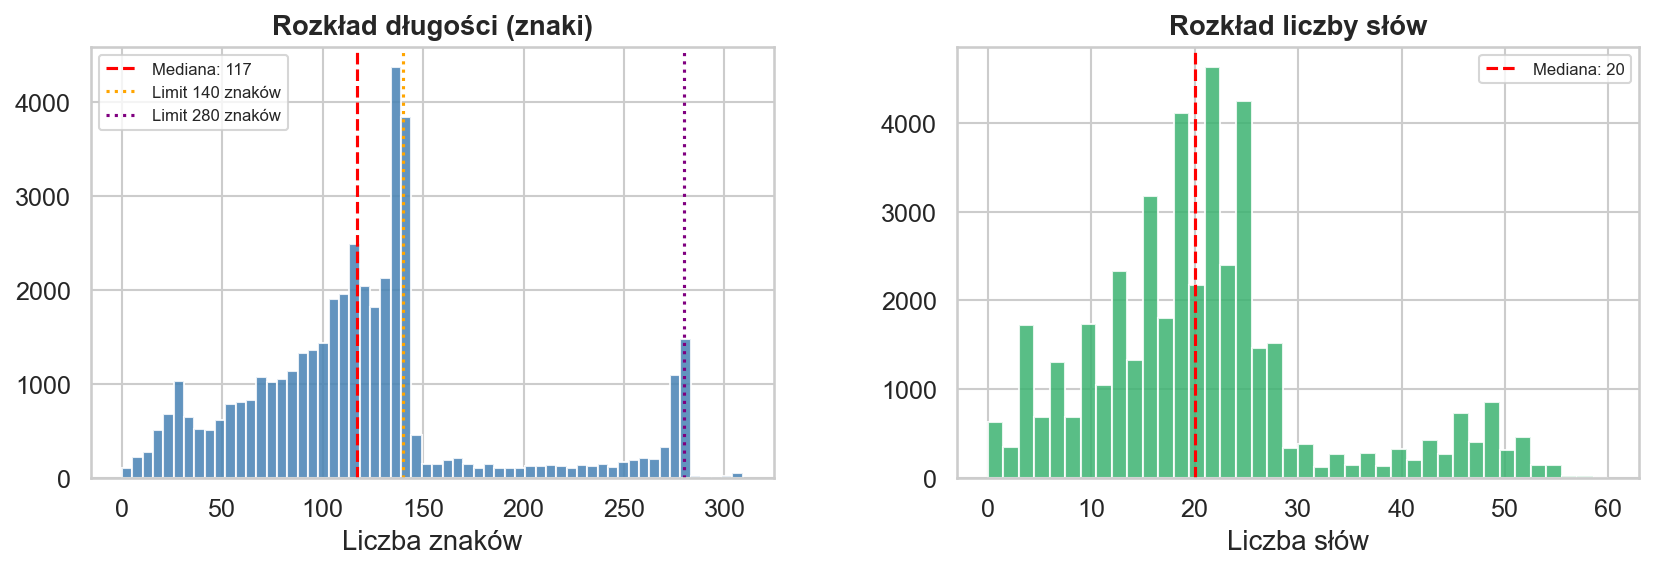
\includegraphics[width=1.05\textwidth]{figures/analysis_tweet_lengths2.png}
    \caption{Rozkład długości tweetów.}
    \label{fig:tweet_length_distribution}
\end{figure}

Na rysunku \ref{fig:tweet_length_distribution} przedstawiono rozkład długości tweetów. Średnia długość wpisu wyniosła około 121 znaków (20,7 słowa), co jest charakterystyczne dla krótkich form publikowanych w serwisie Twitter.

\subsection{Automatyczne generowanie etykiet}

Ze względu na brak ręcznie przygotowanych etykiet emocjonalnych opracowano własny system automatycznego etykietowania danych.

Proces przypisywania etykiet miał charakter hierarchiczny:

\begin{enumerate}
\item NRC Emotion Lexicon,
\item wykrywanie sarkazmu z wykorzystaniem VADER,
\item wykrywanie patriotyzmu na podstawie słów kluczowych,
\item przypisanie klasy neutral.
\end{enumerate}

W pierwszym kroku wykorzystywano NRC Emotion Lexicon, który przypisuje słowom osiem podstawowych emocji: anger, fear, joy, sadness, disgust, surprise, anticipation oraz trust. Następnie stosowano dodatkowe reguły heurystyczne wykrywające sarkazm oraz odniesienia patriotyczne.



\subsection{Rozkład klas emocjonalnych}

Ostatecznie uzyskano zbiór obejmujący jedenaście klas emocjonalnych:

\begin{center}
angry, fearful, joyful, sad, disgusted, surprised, enthusiastic, trusting, sarcastic, patriotic oraz neutral.
\end{center}

\begin{figure}[H]
    \centering
    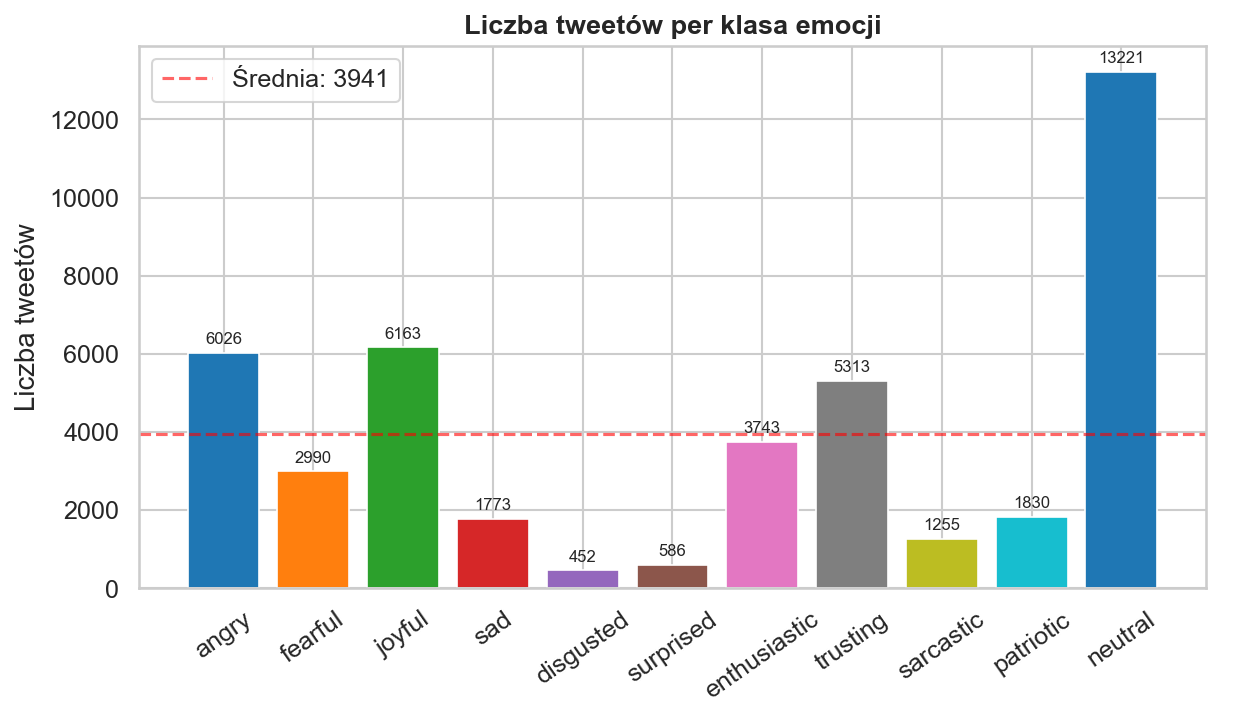
\includegraphics[width=0.97\textwidth]{figures/analysis_class_distribution0.png}
    \caption{Rozkład klas emocjonalnych w zbiorze danych.}
    \label{fig:class_distribution}
\end{figure}
\begin{figure}[H]
    \centering
    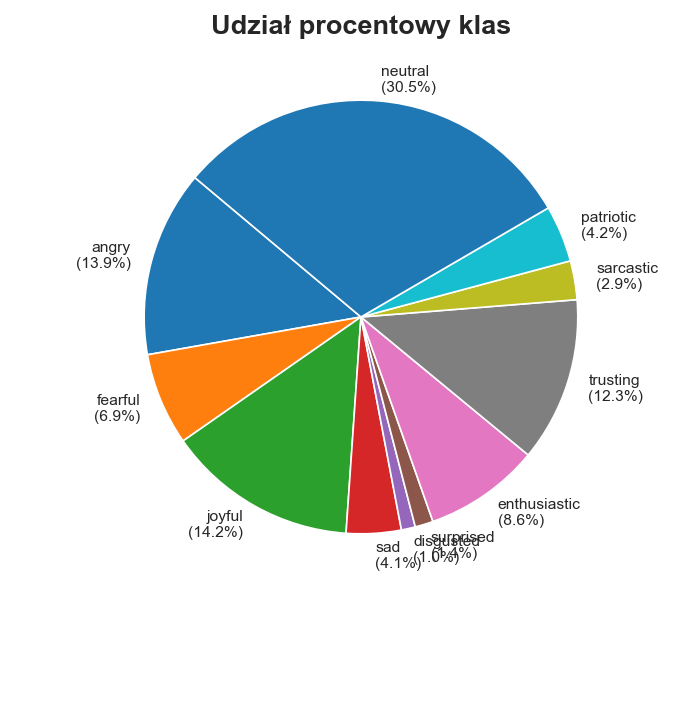
\includegraphics[width=0.77\textwidth]{figures/analysis_class_distribution1.png}
    \caption{Rozkład klas emocjonalnych w zbiorze danych.}
    \label{fig:class_distribution_per}
\end{figure}


Jak pokazano na rysunku \ref{fig:class_distribution}, zbiór danych jest niezbalansowany. Najliczniejszą klasę stanowią tweety neutralne (30,5\%), natomiast klasy disgusted oraz surprised obejmują odpowiednio około 1,0% i 1,4% wszystkich przykładów.

% =====================================================
\section{Zastosowane metody}

W celu oceny różnych sposobów reprezentacji tekstu oraz klasyfikacji emocji przeprowadzono eksperymenty z wykorzystaniem czterech podejść opartych na nowoczesnych metodach przetwarzania języka naturalnego. Zastosowane modele różniły się zarówno sposobem reprezentacji tweetów, jak i architekturą klasyfikatora.

\begin{table}[H]
\centering
\caption{Porównanie zastosowanych podejść.}
\label{tab}
\begin{tabular}{lll}
\toprule
Model & Reprezentacja tekstu & Klasyfikator \\
\midrule
DistilBERT + MLP & embedding CLS (768) & Residual MLP \\
SBERT + MLP & embedding zdania (384) & Residual MLP \\
GloVe + BiLSTM & sekwencja tokenów (200) & BiLSTM + Attention \\
Zero-Shot BART & reprezentacja wewnętrzna BART & NLI (bez treningu) \\
TF-IDF + Logistic Regression & TF-IDF & Logistic Regression \\
\bottomrule
\end{tabular}
\end{table}

\subsection{DistilBERT + MLP}

Pierwsze podejście wykorzystywało embeddingi generowane przez model DistilBERT. Dla każdego tweeta pobierano reprezentację tokenu CLS o wymiarze 768, która stanowiła zagregowany opis całej wypowiedzi.

Embeddingi były następnie przekazywane do wielowarstwowej sieci neuronowej typu MLP (Multi-Layer Perceptron) wyposażonej w połączenia rezydualne (Residual Connections). Zastosowanie połączeń rezydualnych umożliwia stabilniejszy trening głębszych sieci poprzez ułatwienie propagacji gradientów oraz ograniczenie problemu zanikania gradientu.

Architektura składała się z warstwy projekcji wejścia, trzech bloków rezydualnych wykorzystujących funkcję aktywacji GELU oraz końcowej warstwy klasyfikacyjnej przewidującej jedną z jedenastu klas emocjonalnych.

\subsection{SBERT + MLP}

Drugie podejście oparto na modelu Sentence-BERT (SBERT), wykorzystując wariant \texttt{all-MiniLM-L6-v2}. W przeciwieństwie do klasycznego BERT-a, model ten został zaprojektowany do generowania reprezentacji całych zdań i zachowywania podobieństwa semantycznego pomiędzy wypowiedziami.

Każdy tweet reprezentowany był przez wektor o wymiarze 384. Następnie zastosowano tę samą architekturę klasyfikatora MLP z połączeniami rezydualnymi, co w przypadku modelu DistilBERT. Dzięki temu możliwe było bezpośrednie porównanie jakości obu rodzajów embeddingów przy identycznej architekturze klasyfikacyjnej.

\subsection{GloVe + BiLSTM}

Trzecie podejście wykorzystało klasyczne embeddingi GloVe wytrenowane na danych z serwisu Twitter (\texttt{glove-twitter-200}). W przeciwieństwie do modeli transformerowych embeddingi GloVe są statyczne i nie zależą od kontekstu występowania słowa.

Sekwencje tokenów były przetwarzane przez dwukierunkową sieć LSTM (BiLSTM), która analizowała tekst zarówno od początku do końca, jak i w kierunku przeciwnym. Pozwala to lepiej modelować zależności występujące w zdaniu.

Dodatkowo zastosowano mechanizm Additive Attention, którego zadaniem było przypisanie większej wagi najważniejszym fragmentom tweeta. Dzięki temu model mógł koncentrować się na słowach szczególnie istotnych dla określenia emocji, takich jak wyrażenia pozytywne, negatywne lub nacechowane politycznie.

Ostateczna reprezentacja uzyskana przez mechanizm uwagi była przekazywana do warstwy klasyfikacyjnej przewidującej jedną z badanych emocji.

\subsection{Zero-Shot BART}

Ostatnie podejście neuronowe stanowił model \texttt{facebook/bart-large-mnli} wykorzystany w trybie klasyfikacji zero-shot. W odróżnieniu od pozostałych metod model nie był trenowany na zbiorze tweetów Donalda Trumpa.

Klasyfikacja realizowana była poprzez mechanizm Natural Language Inference (NLI). Dla każdego tweeta model oceniał prawdopodobieństwo przypisania do każdej z badanych emocji na podstawie zdań opisujących poszczególne klasy.

Podejście zero-shot stanowiło punkt odniesienia pozwalający ocenić, jak dobrze gotowy model językowy radzi sobie z analizą emocji bez dodatkowego procesu uczenia na danych projektowych.

\subsection{TF--IDF + Logistic Regression}

Oprócz modeli neuronowych wykorzystano również klasyczne podejście oparte na reprezentacji TF--IDF (Term Frequency -- Inverse Document Frequency) oraz regresji logistycznej.

W pierwszym kroku każdy tweet został przekształcony do wektora TF--IDF opisującego częstość występowania słów w dokumencie względem całego korpusu. Reprezentacja ta pozwala uwzględnić znaczenie słów charakterystycznych dla danego tekstu przy jednoczesnym ograniczeniu wpływu bardzo często występujących wyrazów.

Następnie wykorzystano wieloklasową regresję logistyczną, która dla każdej klasy emocjonalnej estymowała prawdopodobieństwo przypisania tweeta do danej kategorii. Model ten stanowił klasyczny punkt odniesienia dla bardziej zaawansowanych metod opartych na embeddingach oraz sieciach neuronowych.

Dodatkową zaletą tego podejścia jest wysoka interpretowalność. Ponieważ każda cecha odpowiada bezpośrednio konkretnemu słowu lub tokenowi, możliwe jest przeprowadzenie szczegółowej analizy wpływu poszczególnych słów na decyzje modelu przy użyciu metody SHAP.

% =====================================================
\section{Wyniki eksperymentów}

\subsection{Porównanie skuteczności modeli}

Tabela \ref{tab:results} przedstawia wartości Accuracy oraz Macro F1 uzyskane przez analizowane modele. Accuracy określa odsetek poprawnie sklasyfikowanych przykładów, natomiast Macro F1 uwzględnia skuteczność dla każdej klasy niezależnie od jej liczności, dzięki czemu lepiej odzwierciedla jakość klasyfikacji w przypadku niezbalansowanych danych.

\begin{table}[H]
\centering
\caption{Porównanie skuteczności modeli.}
\label{tab:results}
\begin{tabular}{lcc}
\toprule
Model & Accuracy & Macro F1 \\
\midrule
DistilBERT + MLP & 0.267 & 0.197 \\
SBERT + MLP & 0.329 & 0.257 \\
GloVe + BiLSTM & 0.518 & 0.443 \\
Zero-Shot BART & 0.132 & 0.121 \\
TF-IDF + Logistic Regression & 0.650 & 0.480 \\
\bottomrule
\end{tabular}
\end{table}

\begin{figure}[H]
\centering

\includegraphics[width=0.95\textwidth]{figures/model_comparison.png}
\caption{Porównanie skuteczności analizowanych modeli.}
\label{fig:model_comparison}
\end{figure}

Najwyższą skuteczność osiągnął model TF-IDF + Logistic Regression, uzyskując Accuracy równą 0.650 oraz Macro F1 na poziomie 0.480. Wśród modeli neuronowych najlepsze wyniki osiągnął model GloVe + BiLSTM z mechanizmem uwagi, który uzyskał Accuracy równą 0.518 oraz Macro F1 równą 0.443.

Model SBERT + MLP osiągnął lepsze wyniki niż DistilBERT + MLP, co sugeruje, że embeddingi projektowane do reprezentowania znaczenia całych zdań lepiej sprawdzają się w zadaniu klasyfikacji emocji. Najsłabsze rezultaty uzyskał model Zero-Shot BART, który nie był trenowany na analizowanym zbiorze danych i pełnił jedynie rolę punktu odniesienia.

\subsection{Analiza skuteczności dla poszczególnych klas}

Sama wartość Accuracy nie pozwala określić, jak dobrze modele radzą sobie z poszczególnymi emocjami. W tym celu przeanalizowano wartości F1-score dla każdej klasy osobno.

\begin{figure}[H]
\centering
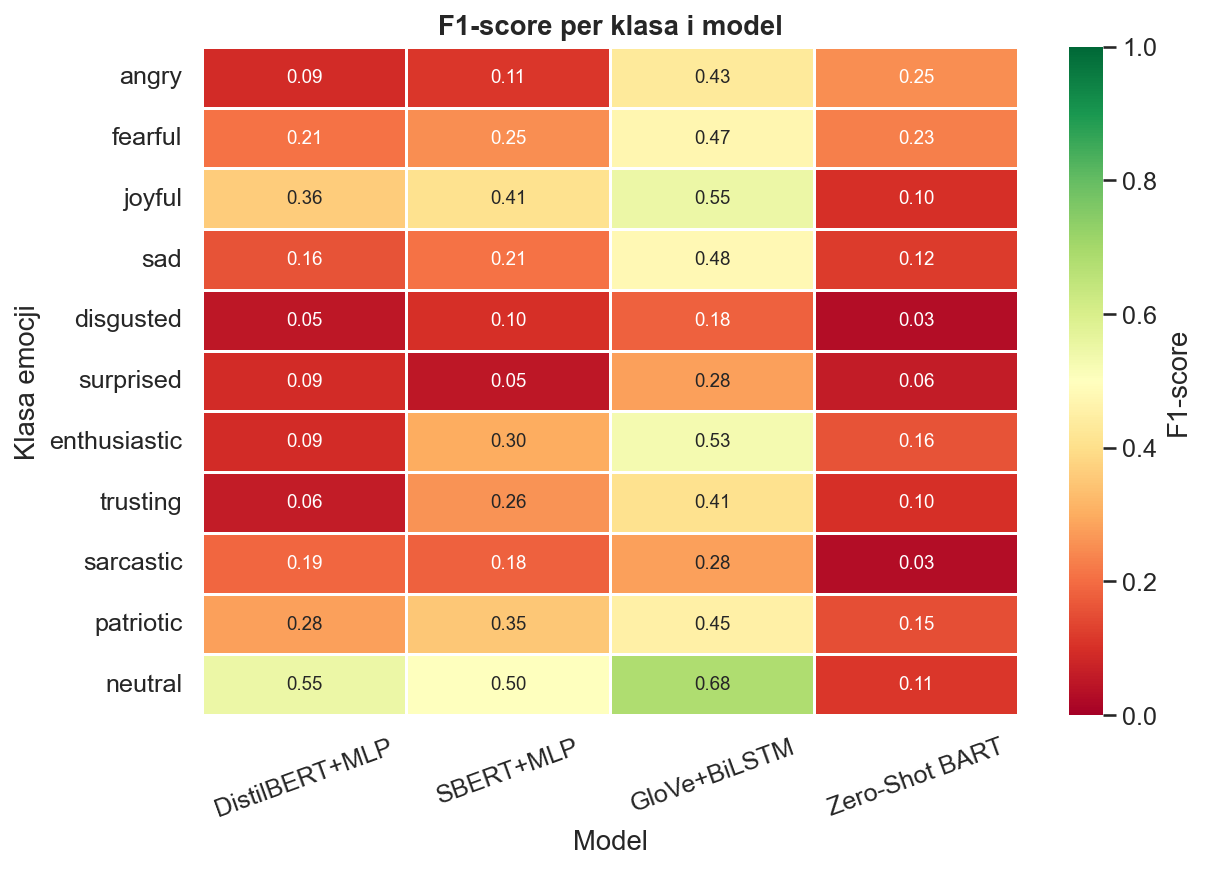
\includegraphics[width=0.95\textwidth]{figures/analysis_f1_per_class2.png}
\caption{Wartości F1-score dla poszczególnych klas emocjonalnych.}
\label{fig:f1_per_class}
\end{figure}

Na rysunku \ref{fig:f1_per_class} przedstawiono wartości F1-score uzyskane dla poszczególnych klas emocjonalnych.

Najlepiej rozpoznawaną klasą była \textit{neutral}, dla której wszystkie modele osiągały relatywnie wysokie wartości F1-score. Dobre wyniki uzyskano również dla klas \textit{joyful} oraz \textit{patriotic}. Emocje te charakteryzują się stosunkowo wyraźnym i powtarzalnym słownictwem, co ułatwia ich identyfikację.

Znacznie większe trudności sprawiały klasy \textit{disgusted}, \textit{surprised} oraz \textit{sarcastic}. Dla tych emocji wszystkie analizowane modele osiągały niskie wartości F1-score, często nieprzekraczające 0.2. Szczególnie trudna okazała się klasa \textit{disgusted}, która była jednocześnie jedną z najmniej licznych klas w całym zbiorze danych.

Widoczna zależność pomiędzy liczebnością klasy a jakością klasyfikacji sugeruje, że niezbalansowany rozkład danych miał istotny wpływ na uzyskane wyniki. Jednocześnie niektóre emocje, takie jak \textit{sarcastic}, pozostają trudne do rozpoznania niezależnie od liczby przykładów, ponieważ ich poprawna identyfikacja często wymaga uwzględnienia szerszego kontekstu wypowiedzi.

Wynik ten jest zgodny z rozkładem danych przedstawionym wcześniej. Klasy posiadające niewielką liczbę przykładów treningowych były znacznie trudniejsze do nauczenia przez modele, co przełożyło się na niższe wartości Precision, Recall oraz F1-score.

\subsection{Analiza błędów klasyfikacji}

Aby lepiej zrozumieć źródła błędów klasyfikacyjnych, przeanalizowano macierz pomyłek dla najlepszego modelu neuronowego, tj. GloVe + BiLSTM.

\begin{figure}[H]
\centering
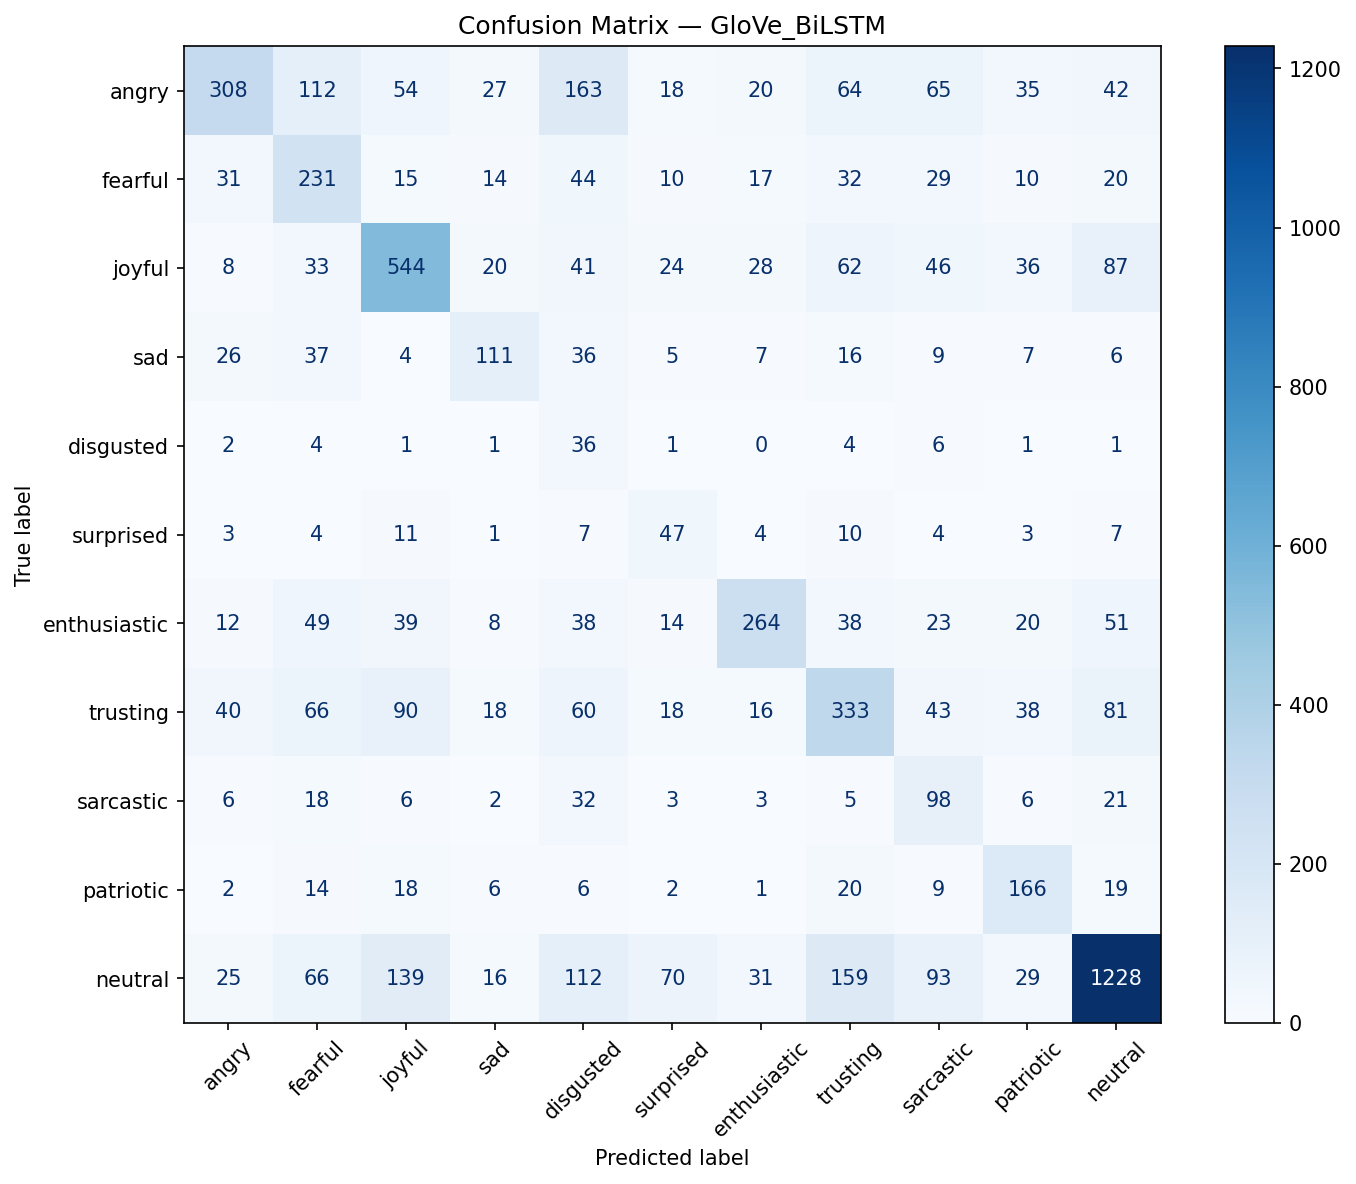
\includegraphics[width=0.9\textwidth]{figures/confusion_matrix_GloVe_BiLSTM.png}
\caption{Macierz pomyłek dla modelu GloVe + BiLSTM.}
\label{fig:confusion_glove}
\end{figure}

Macierz pomyłek przedstawiona na rysunku \ref{fig:confusion_glove} pokazuje, że model najskuteczniej rozpoznaje klasy licznie reprezentowane w zbiorze danych, takie jak \textit{neutral}, \textit{joyful}, \textit{angry} oraz \textit{trusting}. Jednocześnie można zauważyć wyraźną tendencję do przewidywania klasy \textit{neutral}, która była najczęściej występującą kategorią w całym zbiorze danych.

Analiza błędnych klasyfikacji wskazuje również na występowanie pomyłek pomiędzy emocjami o podobnym znaczeniu semantycznym. Przykładowo klasa \textit{angry} była często mylona z klasami \textit{fearful} oraz \textit{disgusted}, natomiast klasa \textit{trusting} była regularnie klasyfikowana jako \textit{joyful} lub \textit{neutral}. Takie błędy są częściowo zrozumiałe, ponieważ granice pomiędzy niektórymi emocjami nie są jednoznaczne nawet dla człowieka.

Największe problemy dotyczyły klas rzadkich, takich jak \textit{disgusted}, \textit{surprised} oraz \textit{sarcastic}. Dla tych kategorii liczba poprawnych predykcji była relatywnie niewielka, a wiele przykładów przypisywano do klas częstszych. Jest to typowy efekt niezbalansowanego zbioru danych, w którym model otrzymuje znacznie mniej przykładów umożliwiających nauczenie charakterystycznych wzorców dla klas mniejszościowych.

Wyniki potwierdzają, że głównym źródłem błędów była zarówno nierównowaga klas, jak i częściowe nakładanie się znaczeniowe niektórych emocji występujących w tweetach.

% =====================================================
% =====================================================
\section{Analiza SHAP}

Jednym z celów projektu było zbadanie interpretowalności zastosowanych modeli. W tym celu wykorzystano metodę SHAP (SHapley Additive exPlanations), która pozwala określić wpływ poszczególnych cech wejściowych na decyzję klasyfikatora.

Analizę przeprowadzono dla dwóch istotnie różnych podejść: modelu wykorzystującego embeddingi zdań (SBERT + MLP) oraz modelu TF--IDF + Logistic Regression. Pozwoliło to porównać nie tylko skuteczność modeli, ale również możliwość wyjaśnienia ich decyzji.

\subsection{Model SBERT + MLP}

W przypadku modelu SBERT + MLP wejściem klasyfikatora był embedding zdania o wymiarze 384. Oznacza to, że SHAP analizował wpływ poszczególnych wymiarów reprezentacji wektorowej, a nie konkretnych słów występujących w tweecie.

\begin{figure}[H]
\centering

\includegraphics[width=0.75\textwidth]{figures/shap_summary_SBERT_MLP_class0.png}
\caption{Najważniejsze cechy według SHAP dla modelu SBERT + MLP dla klasy angry.}
\label{fig:shap_sbert}
\end{figure}

Jak pokazano na rysunku \ref{fig:shap_sbert}, SHAP identyfikuje grupę wymiarów embeddingu, które mają największy wpływ na przypisanie klasy \textit{angry}. Możliwe jest określenie względnego znaczenia poszczególnych cech, jednak ich interpretacja pozostaje utrudniona.

Poszczególne wymiary embeddingu nie posiadają jednoznacznego znaczenia semantycznego. W przeciwieństwie do klasycznych cech tekstowych nie można stwierdzić, które konkretne słowa lub konstrukcje językowe odpowiadają za obserwowany wpływ. W rezultacie analiza SHAP pozwala ocenić, które fragmenty reprezentacji wektorowej są istotne dla modelu, ale nie wyjaśnia bezpośrednio mechanizmu podejmowania decyzji.

Wynik ten dobrze ilustruje jedną z głównych cech nowoczesnych reprezentacji embeddingowych. Oferują one bogaty opis semantyczny tekstu, jednak odbywa się to kosztem interpretowalności.

\subsection{Model TF--IDF + Logistic Regression}

Znacznie bardziej intuicyjne wyniki uzyskano dla modelu TF--IDF + Logistic Regression. W tym przypadku każda cecha odpowiada konkretnemu słowu występującemu w zbiorze danych, dzięki czemu wartości SHAP mogą być interpretowane bezpośrednio w kontekście treści tweetów.

\begin{figure}[H]
\centering

\includegraphics[width=0.75\textwidth]{figures/shap_tfidf_baseline_class2.png}
\caption{Najważniejsze słowa wpływające na klasyfikację klasy \textit{joyful}.}
\label{fig:shap_joyful}
\end{figure}

\begin{figure}[H]
\centering

\includegraphics[width=0.75\textwidth]{figures/shap_tfidf_baseline_class0.png}
\caption{Najważniejsze słowa wpływające na klasyfikację klasy \textit{angry}.}
\label{fig:shap_angry}
\end{figure}

Dla klasy \textit{joyful} (rysunek \ref{fig:shap_joyful}) największy pozytywny wpływ miały słowa takie jak \textit{love}, \textit{hope}, \textit{thanks}, \textit{great}, \textit{good} oraz \textit{wonderful}. Wszystkie są naturalnie kojarzone z pozytywnym wydźwiękiem emocjonalnym, co sugeruje, że model nauczył się wykorzystywać intuicyjne sygnały językowe obecne w danych.

Podobną zależność można zaobserwować dla klasy \textit{angry} (rysunek \ref{fig:shap_angry}). Wysokie dodatnie wartości SHAP uzyskały słowa takie jak \textit{bad}, \textit{fight}, \textit{illegal} czy \textit{vote}. Są to wyrażenia często pojawiające się w kontekście konfliktu, krytyki lub sporów politycznych, a więc naturalnie związane z emocjami negatywnymi.

Interesującą obserwacją jest również fakt, że dla klasy \textit{angry} silnie ujemne wartości SHAP uzyskały słowa \textit{thank}, \textit{thanks}, \textit{great} oraz \textit{best}. Oznacza to, że ich obecność zmniejszała prawdopodobieństwo przypisania tej klasy. Jest to zgodne z intuicją, ponieważ słowa te występowały częściej w tweetach oznaczonych jako \textit{joyful}, \textit{trusting} lub \textit{patriotic}.

W przeciwieństwie do modelu SBERT możliwe było więc nie tylko wskazanie ważnych cech, ale również bezpośrednie zrozumienie, dlaczego model podjął określoną decyzję.

\subsection{Najważniejsze obserwacje}

Analiza SHAP ujawniła wyraźną różnicę pomiędzy interpretowalnością badanych modeli.

Model SBERT wykorzystywał złożoną reprezentację semantyczną tekstu, jednak wpływ poszczególnych wymiarów embeddingu był trudny do przełożenia na język naturalny. Z kolei model TF--IDF pozwalał bezpośrednio wskazać słowa odpowiedzialne za przypisanie danej emocji, dzięki czemu jego decyzje były znacznie bardziej przejrzyste.

Warto zauważyć, że najważniejsze słowa wskazane przez SHAP były zgodne z intuicją oraz charakterem analizowanych emocji. Sugeruje to, że model nie opierał się na przypadkowych korelacjach, lecz rzeczywiście wykorzystywał sygnały językowe związane z treścią tweetów.

Ostatecznie analiza SHAP pokazała, że wzrost złożoności reprezentacji tekstu prowadzi do spadku interpretowalności modelu. Jest to klasyczny kompromis pomiędzy możliwością wyjaśnienia decyzji a wykorzystaniem bardziej abstrakcyjnych reprezentacji semantycznych.


% =====================================================
\section{Dyskusja wyników}

\subsection{Dlaczego GloVe + BiLSTM osiągnął najlepsze wyniki wśród modeli neuronowych?}

Jednym z najbardziej interesujących wyników eksperymentów jest wyraźna przewaga modelu GloVe + BiLSTM nad modelami wykorzystującymi embeddingi transformerowe. Jak pokazano w tabeli \ref{tab:results}, model ten osiągnął Accuracy równą 0.518, podczas gdy DistilBERT + MLP uzyskał jedynie 0.267.

Na pierwszy rzut oka wynik ten może wydawać się zaskakujący. DistilBERT jest znacznie bardziej zaawansowanym modelem językowym niż klasyczne embeddingi GloVe, jednak w przeprowadzonym eksperymencie wykorzystano jedynie gotowy embedding CLS przekazywany następnie do klasyfikatora MLP. W takiej konfiguracji model operuje na pojedynczym wektorze reprezentującym cały tweet i nie wykorzystuje informacji o kolejności słów.

Model GloVe + BiLSTM działał w odmienny sposób. BiLSTM przetwarzał pełną sekwencję tokenów, dzięki czemu mógł modelować lokalne zależności pomiędzy słowami. Dodatkowo zastosowany mechanizm Attention pozwalał koncentrować się na fragmentach wypowiedzi najbardziej istotnych dla rozpoznawanej emocji.

Istotnym czynnikiem mogła być również domena danych wykorzystanych podczas uczenia embeddingów. Model \texttt{glove-twitter-200} został wytrenowany bezpośrednio na tweetach, przez co lepiej odwzorowuje charakterystyczny język mediów społecznościowych, obejmujący skróty, niestandardową interpunkcję czy częste użycie wielkich liter. Analizowane tweety są znacznie bliższe temu środowisku niż tekstom wykorzystywanym podczas trenowania DistilBERT.

Wyniki sugerują więc, że w analizowanym zadaniu większe znaczenie miało dopasowanie reprezentacji do domeny oraz możliwość modelowania sekwencji niż sama złożoność modelu językowego.

\subsection{Dlaczego model Zero-Shot BART osiągnął tak słabe wyniki?}

Najsłabsze rezultaty uzyskał model Zero-Shot BART, którego Accuracy wyniosła jedynie 0.132. Wynik ten był znacząco niższy od wszystkich pozostałych metod.

Jednym z powodów może być sposób działania klasyfikacji zero-shot. Model \texttt{bart-large-mnli} nie był trenowany do rozpoznawania emocji w tweetach, lecz do zadania Natural Language Inference. Ocenia on, czy zdanie opisujące daną emocję jest zgodne z treścią tweeta. W praktyce oznacza to, że musi samodzielnie interpretować znaczenie etykiet takich jak \textit{patriotic}, \textit{sarcastic} czy \textit{enthusiastic}, mimo że nie były one częścią procesu treningowego.

Dodatkową trudność stanowi specyfika tweetów Donalda Trumpa. Wiele wpisów zawiera jednocześnie elementy kilku emocji, co utrudnia jednoznaczne przypisanie pojedynczej klasy. Przykładowo wypowiedź krytykująca przeciwników politycznych może zawierać zarówno cechy klasy \textit{angry}, jak i \textit{patriotic}.

Wyniki pokazują, że mimo dużych możliwości współczesnych modeli językowych klasyfikacja emocji pozostaje zadaniem silnie zależnym od domeny danych i wymaga dostosowania modelu do konkretnego problemu.

\subsection{Najtrudniejsze emocje do rozpoznania}

Analiza wartości F1-score dla poszczególnych klas (rysunek \ref{fig:f1_per_class}) pokazuje, że poziom trudności klasyfikacji był bardzo nierównomierny.

Najlepiej rozpoznawaną klasą była \textit{neutral}, dla której średni F1-score wyniósł około 0.46. Relatywnie wysokie wyniki osiągano również dla klas \textit{joyful} oraz \textit{patriotic}. Wspólną cechą tych kategorii jest występowanie charakterystycznego słownictwa, które modele mogły stosunkowo łatwo powiązać z konkretną etykietą.

Znacznie większe trudności sprawiały klasy \textit{disgusted} (średni F1 = 0.09), \textit{surprised} (0.12) oraz \textit{sarcastic} (0.17). Wyniki te pozostawały niskie niezależnie od zastosowanej architektury.

W przypadku klas \textit{disgusted} i \textit{surprised} istotnym problemem była niewielka liczba przykładów treningowych. Jak pokazano wcześniej na rysunkach \ref{fig:class_distribution} oraz \ref{fig:class_distribution_per}, klasy te stanowiły około 1% całego zbioru danych. Tak mała reprezentacja utrudnia modelom nauczenie stabilnych wzorców klasyfikacyjnych.

Szczególnym przypadkiem pozostaje sarkazm. W przeciwieństwie do większości emocji jego identyfikacja często wymaga wiedzy o kontekście wypowiedzi lub intencji autora. Informacje te nie były dostępne dla analizowanych modeli, dlatego rozpoznawanie sarkazmu okazało się trudne niezależnie od wykorzystanej reprezentacji tekstu.

\subsection{Ograniczenia przeprowadzonych eksperymentów}

Interpretując uzyskane wyniki należy pamiętać, że analizowany zbiór nie zawierał ręcznie przygotowanych etykiet emocjonalnych. Wszystkie klasy zostały wygenerowane automatycznie na podstawie słowników emocji i dodatkowych reguł heurystycznych.

Oznacza to, że część wyników odzwierciedla skuteczność odtwarzania procesu etykietowania, a niekoniecznie rzeczywistego rozpoznawania emocji przez modele. Widać to szczególnie w analizie SHAP dla modelu TF--IDF, gdzie największy wpływ na decyzje klasyfikatora miały słowa bezpośrednio związane z przypisywaniem etykiet.

Pomimo tego ograniczenia przeprowadzone eksperymenty pozwoliły porównać kilka istotnie różnych podejść do reprezentacji tekstu oraz pokazały, jak zmienia się interpretowalność modeli wraz ze wzrostem ich złożoności.



% =====================================================
\section{Wnioski}

Celem projektu było zbudowanie modelu analizy emocji dla tweetów Donalda Trumpa oraz zbadanie interpretowalności różnych podejść do reprezentacji tekstu przy użyciu metody SHAP.

Na podstawie przeprowadzonych eksperymentów można sformułować następujące wnioski:

\begin{enumerate}
\item \textbf{Najwyższą skuteczność osiągnął model TF--IDF + Logistic Regression}, uzyskując Accuracy równą 0.650 oraz Macro F1 równą 0.480.

\item \textbf{Spośród modeli neuronowych najlepsze wyniki uzyskał model GloVe + BiLSTM z mechanizmem Attention} (Accuracy = 0.518, Macro F1 = 0.443), przewyższając modele wykorzystujące zamrożone embeddingi transformerowe.

\item \textbf{Klasyfikacja emocji okazała się szczególnie trudna dla klas rzadkich.} Najniższe wartości F1-score uzyskano dla emocji \textit{disgusted}, \textit{surprised} oraz \textit{sarcastic}, podczas gdy najlepiej rozpoznawane były klasy \textit{neutral}, \textit{joyful} i \textit{patriotic}.

\item \textbf{Analiza SHAP potwierdziła wyraźną różnicę w interpretowalności pomiędzy modelami.} W przypadku modelu TF--IDF możliwe było bezpośrednie wskazanie słów wpływających na decyzję klasyfikatora, natomiast dla modeli opartych na embeddingach interpretacja ograniczała się do analizy poszczególnych wymiarów reprezentacji wektorowych.

\item \textbf{Uzyskane wyniki należy interpretować z uwzględnieniem sposobu tworzenia etykiet.} Zastosowana procedura automatycznej anotacji umożliwiła przygotowanie dużego zbioru treningowego, jednak mogła również wpływać na końcową skuteczność modeli.

\end{enumerate}

Przeprowadzona analiza pokazała, że w badanym problemie klasyczne metody reprezentacji tekstu pozostają konkurencyjne wobec bardziej złożonych podejść neuronowych. Jednocześnie wyniki potwierdzają, że skuteczność modelu zależy nie tylko od zastosowanej architektury, ale również od charakterystyki danych, jakości etykiet oraz stopnia dopasowania reprezentacji tekstu do analizowanej domeny.

W przyszłych pracach warto rozważyć wykorzystanie ręcznie anotowanego zbioru danych oraz pełny fine-tuning modeli transformerowych. Pozwoliłoby to dokładniej ocenić potencjał nowoczesnych modeli językowych w zadaniu klasyfikacji emocji oraz ograniczyć wpływ błędów wynikających z automatycznego etykietowania.





% =====================================================

\section*{Repozytorium}

\bigskip

Ze względu na ograniczoną objętość raportu przedstawiono jedynie najważniejsze wyniki oraz przykładowe wizualizacje. Większa analiza eksperymentów, obejmująca dodatkowe wykresy, przebiegi uczenia modeli, macierze pomyłek, wyniki dla poszczególnych klas emocjonalnych oraz kompletne analizy SHAP, została udostępniona w notatniku Jupyter \textit{analiza\_wynikow.ipynb} znajdującym się w repozytorium projektu.

Kod źródłowy projektu:

\url{https://github.com/martynalacha/Trump-Tweet-Emotion-Classifier/tree/main}

\bigskip

Autorzy:

\begin{itemize}
\item Martyna Lach
\item Julia Mucha
\item Piotr Waszak
\end{itemize}

\end{document}
